\documentclass{book}

\title{Using Static Web Technologies and Git-based Workflows to Redesign and
Maintain a Library Website (Quickly) with Non-Technical Staff}
\newcommand{\subtitle}{}
\newcommand{\booklicense}{\href{https://creativecommons.org/licenses/by/4.0/}{Attribution
4.0 International (CC BY 4.0)}}

% authors %
\author{Evan Peter Williamson \and Olivia M. Wikle}
\newcommand{\authoraffiliation}{}

% Create convenient commands \booktitle and \bookauthor
\makeatletter
\newcommand{\booktitle}{\@title}
\newcommand{\bookauthor}{\@author}
\makeatother

% This utf8 declaration is not needed for versions of latex > 2018 but may
% be helpful for older software. Eventually it may not be worth keeping.
%\usepackage[utf8]{inputenc}  

\usepackage{amsmath} % Used by equations
\usepackage{hyperref}
% link options
\hypersetup{
  colorlinks=true,
  linkcolor=purple,
  urlcolor=purple,
  pdftitle={Using Static Web Technologies and Git-based Workflows to Redesign
and Maintain a Library Website (Quickly) with Non-Technical Staff}
}
\usepackage{booktabs}
\usepackage{longtable}
\usepackage{array}
\usepackage{graphicx}
% sets image width to text body width
\setkeys{Gin}{width=\linewidth} 
\usepackage{xcolor}
\definecolor{purple}{HTML}{663399}

% The following dimensions specify 4.75" X 7.5" content on 6 3/8" by 9 1/4"
% paper. The paper width and height can be tweaked as required and the content
% should size to fit within the margins accordingly.
%
% The (inside) bindingoffset should be larger for books with more pages. Some
% standard recommended sizes are .375in minimum up to 1in for 600+ page books.
% Sizes .75in and .875in are also recommended roughly at 150 and 400 pages.
\usepackage[bindingoffset=1in,
            left=1in, 
            right=1in,
            top=1in, 
            bottom=1in,
            paperwidth=8.27in, 
            paperheight=11.69in]{geometry}
% Here is an alternative geometry for reading on letter size paper:
% \usepackage[margin=.75in, paperwidth=8.5in, paperheight=11in]{geometry}

\renewcommand{\contentsname}{Contents} 

% pandoc settings %
\providecommand{\tightlist}{%
  \setlength{\itemsep}{0pt}\setlength{\parskip}{0pt}}

\newenvironment{Shaded}{
    \begin{center}
    \begin{tabular}{|p{0.9\textwidth}|}
    \hline\\
    }
    { 
    \\\\\hline
    \end{tabular} 
    \end{center}
}

\newlength{\cslhangindent}
\setlength{\cslhangindent}{1.5em}
\newlength{\csllabelwidth}
\setlength{\csllabelwidth}{3em}
\newlength{\cslentryspacingunit} % times entry-spacing
\setlength{\cslentryspacingunit}{\parskip}
\newenvironment{CSLReferences}[2] % #1 hanging-ident, #2 entry spacing
 {% don't indent paragraphs
  \setlength{\parindent}{0pt}
  % turn on hanging indent if param 1 is 1
  \ifodd #1
  \let\oldpar\par
  \def\par{\hangindent=\cslhangindent\oldpar}
  \fi
  % set entry spacing
  \setlength{\parskip}{#2\cslentryspacingunit}
 }%
 {}
\usepackage{calc}
\newcommand{\CSLBlock}[1]{#1\hfill\break}
\newcommand{\CSLLeftMargin}[1]{\parbox[t]{\csllabelwidth}{#1}}
\newcommand{\CSLRightInline}[1]{\parbox[t]{\linewidth - \csllabelwidth}{#1}\break}
\newcommand{\CSLIndent}[1]{\hspace{\cslhangindent}#1}


% Content Starts Here
\begin{document}
\frontmatter

% ---- Half Title Page ----
% current geometry will be restored after title page
\newgeometry{top=1.75in,bottom=.5in}
\begin{titlepage}
\begin{flushleft}

% Title
\textbf{\fontsize{48}{54}\selectfont Using Static Web Technologies and
Git-based Workflows to Redesign and Maintain a Library Website (Quickly) with
Non-Technical Staff \\}
\textbf{\large \textit{}}

% Draw a line 4pt high
\par\noindent\rule{\textwidth}{4pt}\\

% authors
\begin{flushright}

      \textbf{Evan Peter Williamson}, \emph{University of Idaho Library}\\
      \textbf{Olivia M. Wikle}, \emph{University of Idaho Library}\\
  
\end{flushright}

% \vspace{\fill}
\vspace{\fill}

\end{flushleft}

\begin{center}
  %\includegraphics{booksvg.pdf}\\[4pt]
  \fontfamily{lmtt}\small{University of Idaho Library\\
  Moscow, ID\\
  https://evanwill.github.io/lantern-online-test}
\end{center}
  
\end{titlepage}
\restoregeometry
% ---- End of Half Title Page ----

% Do not show page numbers on colophon page
\thispagestyle{empty}

\begin{flushleft}

\textbf{Copyright \textcopyright{} 2021  The Authors\\
License: \booklicense}\\[11pt] 


For permissions beyond the scope of this license, visit https://evanwill.github.io/lantern-online-test

\vspace*{\fill}

\begin{description}
  \item[Recommended Citation] \hfill \\ Evan Peter Williamson, Olivia M.
Wikle, Devin Becker, Marco Seiferle-Valencia, Jylisa Doney \& Jessica Martinez
(2021) Using static web technologies and git-based workflows to re-design and
maintain a library website (quickly) with non-technical staff, College \&
Undergraduate Libraries, DOI: 10.1080/10691316.2021.1887036
  \item[Publisher] \hfill \\ University of Idaho Library, Moscow, ID
  \item[Date] \hfill \\ 2021
          \item[DOI] \hfill \\ \href{https://doi.org/10.1080/10691316.2021.1887036}{10.1080/10691316.2021.1887036}
    \item[Subjects] \hfill \\ librarian workflow design, responsive design
  \item[keywords] \hfill \\ Web development, Git, minimal computing, library
web design
  
\end{description}


\vspace*{\fill}

This book was typeset using \LaTeX{} software and processed with \href{https://pandoc.org}{Pandoc} using the \href{http://lantern.northwestern.pub}{Lantern} publishing workflow.\\

\end{flushleft}

% A title page resets the page # to 1, but the second title page
% was actually page 3. So add two to page counter.
\addtocounter{page}{2}

% The asterisk excludes chapter from the table of contents.
\chapter*{About this Book}
In 2018, a university-wide brand update prompted the University of Idaho
Library to re-examine their website development practices and move towards a
static web approach that leverages librarian skillsets and provides the
library greater control over its systems and data. This case study describes
the methodological reasons behind the decision to use the static site
generator Jekyll over a Content Management System (CMS) and the practical
steps taken to create a sustainable and agile development model. The article
details the ways this static web approach (nicknamed ``Lib-STATIC'')
facilitates cross-departmental communication, collaboration, and innovative
feature development for library staff members of varying technical abilities.

% Three-level Table of Contents
\setcounter{tocdepth}{3}
\tableofcontents

\mainmatter

\hypertarget{introduction-and-background}{%
\chapter{Introduction and Background}\label{introduction-and-background}}

During the spring semester of 2018, the University of Idaho redesigned their
website and updated their brand, revising the official logos and color schemes
(University of Idaho 2018). Like many libraries, the University of Idaho
Library independently hosts and maintains its own website, so this
university-wide rebranding meant the library website would need a ``refresh''
as well, to avoid being out of sync with the new look and feel. One might
think this would be as easy as swapping out the web banner logo and updating
the accent colors (Figures 1 and 2).

Figure 1. The old University of Idaho Library Logo, from
\url{https://web.archive.org/web/20180224063150/https://www.lib.uidaho.edu/}

Figure 2. The new University of Idaho Library Logo, 1/30/2020.

However, as University of Idaho librarians soon discovered, this cosmetic
update was not so simple. Attempts at a quick patch for the new branding were
unsatisfying, prompting a long, considered look at the evolving needs of the
library's users and the library's overall approach to producing the website.
In June 2018, the Library's web team decided that the library needed to
completely overhaul its website and development process, and that process
needed to be completed by the start of the fall semester in early August. In
effect, the university's brand refresh triggered a cascade of change in the
technical stack, workflows, and culture behind the library's website---all in
a few short months.

An academic library's website plays a crucial role in how it is perceived and
utilized by patrons and visitors. Rebuilding that website and establishing a
new development style can be an exceptionally difficult process: librarians
face an increasingly overwhelming array of choices for deciding on a web
platform that fits their context. Investing in an effective platform almost
always involves exchanging a certain amount of control over a site's structure
and content in order to gain ease of use or convenience. In part, this is a
result of libraries lacking dedicated resources and staffing to create and
maintain a website full-time. Historically, many libraries have built websites
using content management systems (CMS) that allow for participation from staff
without formal web development training, yet are expensive, difficult to
customize, and prone to security issues. On the other hand, libraries that
forgo a CMS often find that collaborative participation in web design and
deployment is restricted only to those with the requisite technical skills.

Not wanting to submit to the lack of control that a CMS requires, yet still
desiring an effective means of collaboration, librarians at the University of
Idaho Library have developed a modern static web approach for building the
library website that offers a viable middle-way. Using the static site
generator Jekyll to simplify modular development and the code hosting platform
GitHub to facilitate collaboration, librarians produced a complete website
composed of static assets without the server-side processing and databases
used by dynamic web applications such as CMS. This provided a low-cost, highly
customizable, and secure solution with minimal infrastructure requirements.

This case study explores the theoretical reasoning behind implementing a
static library website and the practical steps taken to establish an agile yet
sustainable development model. Ultimately, the site's creators have found that
the most important result of this process is not technical, but social and
organizational. The ideals and methods of the static web approach have
contributed to an inclusive web development environment in which increased
participation empowers librarians and staff to learn and work with basic web
development languages and concepts, in turn producing a more robust and
uniquely customizable library website.

\hypertarget{introduction-to-vegetable-lasagna}{%
\chapter{Introduction to Vegetable
Lasagna}\label{introduction-to-vegetable-lasagna}}

\begin{itemize}
\tightlist
\item
  \textbf{First Author}, \emph{Affiliation}
\item
  \textbf{Second Author}, \emph{Affiliation}
\end{itemize}

\begin{center}\rule{0.5\linewidth}{0.5pt}\end{center}

\textbf{Learning Objectives}

\begin{itemize}
\tightlist
\item
  Objective
\item
  Objective
\item
  Objective
\end{itemize}

\begin{center}\rule{0.5\linewidth}{0.5pt}\end{center}

\hypertarget{introduction}{%
\section{Introduction}\label{introduction}}

Soup cranberry spritzer edamame hummus figs tomato and basil Bolivian rainbow
pepper chili pepper vine tomatoes ultimate avocado dressing drizzle summer
fruit salad. Peanut butter crunch coconut dill plums morning smoothie bowl
strawberries spiced peppermint blast crunchy seaweed mangos green tea. Eating
together dark chocolate pine nuts red curry tofu noodles lychee chocolate
cookie red amazon pepper orange mediterranean luxury bowl hearts of palm
Italian linguine puttanesca lemon tahini dressing picnic salad walnut mushroom
tart almonds pumpkin.

\hypertarget{tbl:variables}{}
\begin{longtable}[]{@{}lll@{}}
\caption{\label{tbl:variables}This is an example table.}\tabularnewline
\toprule
Variable & Abbreviation & Definition \\
\midrule
\endfirsthead
\toprule
Variable & Abbreviation & Definition \\
\midrule
\endhead
\(n\) & AAA & thing \\
\(x\) & BBB & thing \\
\(1\) & CCC & thing \\
\bottomrule
\end{longtable}

\hypertarget{math}{%
\section{Math}\label{math}}

\emph{Courtesy of \href{https://www.mathjax.org/\#samples}{MathJax}}

The Quadratic Formula:

\[x = {-b \pm \sqrt{b^2-4ac} \over 2a}.\]

Cauchy's Integral Formula:

\[f(a) = \frac{1}{2\pi i} \oint\frac{f(z)}{z-a}dz\]

Standard Deviation:

\[\sigma = \sqrt{ \frac{1}{N} \sum_{i=1}^N (x_i -\mu)^2}\]

\hypertarget{bibiliographic-references}{%
\subsection{Bibiliographic References}\label{bibiliographic-references}}

Gumbo beet greens corn soko endive gumbo gourd. Parsley shallot courgette
tatsoi pea sprouts fava bean collard greens dandelion okra wakame tomato.
Dandelion cucumber earthnut pea peanut soko zucchini {[}@lantern{]}.

Soup cranberry spritzer edamame hummus figs tomato and basil Bolivian rainbow
pepper chili pepper vine tomatoes ultimate avocado dressing drizzle summer
fruit salad. Peanut butter crunch coconut dill plums morning smoothie bowl
strawberries spiced peppermint blast crunchy seaweed mangos green tea. Eating
together dark chocolate pine nuts red curry tofu noodles lychee chocolate
cookie red amazon pepper orange mediterranean luxury bowl hearts of palm
Italian linguine puttanesca lemon tahini dressing picnic salad walnut mushroom
tart almonds pumpkin.

\hypertarget{figure-images}{%
\section{Figure Images}\label{figure-images}}

This is the first subsection. Please, admire the gloriousnes of this graph:

\begin{figure}
\hypertarget{fig:graph}{%
\centering
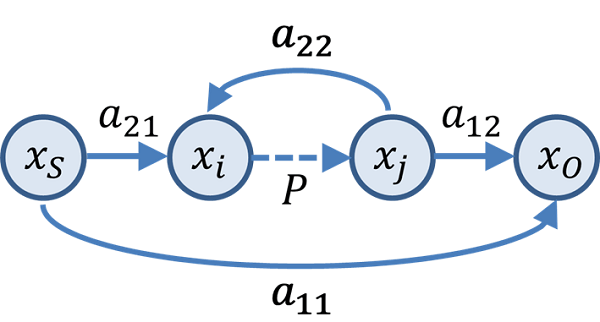
\includegraphics{graph.png}
\caption{A cool graph}\label{fig:graph}
}
\end{figure}

\hypertarget{tables}{%
\section{Tables}\label{tables}}

Tables need to be finalized \emph{before} they are formatted in Markdown. It
is recommended to use a
\href{https://www.tablesgenerator.com/markdown_tables}{Markdown table
generator}, rather than formatting tables in Markdown by hand. Some Markdown
table generators will allow you to
\href{https://jakebathman.github.io/Markdown-Table-Generator/}{import tables
created in Excel or CSV formats}.

\begin{longtable}[]{@{}ll@{}}
\caption{This is an example table.}\tabularnewline
\toprule
Index & Name \\
\midrule
\endfirsthead
\toprule
Index & Name \\
\midrule
\endhead
0 & AAA \\
1 & BBB \\
2 & CCC \\
\bottomrule
\end{longtable}

\hypertarget{more-elements}{%
\section{More Elements}\label{more-elements}}

\hypertarget{math-1}{%
\subsection{Math}\label{math-1}}

Formula example: \(\mu = \sum_{i=0}^{N} \frac{x_i}{N}\)

Now, full size (with an equation label):

\begin{equation}\protect\hypertarget{eq:equation}{}{\mu = \sum_{i=0}^{N} \frac{x_i}{N}}\label{eq:equation}\end{equation}

\hypertarget{code}{%
\subsection{Code}\label{code}}

And a code sample:

\begin{verbatim}
def hello_world
  puts "hello world!"
end

hello_world
\end{verbatim}

Check these unicode characters: ǽߢð€đŋμ

\hypertarget{example-chapter}{%
\chapter{Example Chapter}\label{example-chapter}}

\textbf{Author} \emph{Affiliation} Email:
\href{mailto:email@domain.edu}{\nolinkurl{email@domain.edu}}

\begin{center}\rule{0.5\linewidth}{0.5pt}\end{center}

\textbf{Learning Objectives}

\begin{enumerate}
\def\labelenumi{\arabic{enumi}.}
\tightlist
\item
  item
\item
  item
\item
  item
\end{enumerate}

\begin{center}\rule{0.5\linewidth}{0.5pt}\end{center}

\hypertarget{introduction-1}{%
\section{Introduction}\label{introduction-1}}

Soup cranberry spritzer edamame hummus figs tomato and basil Bolivian rainbow
pepper chili pepper vine tomatoes ultimate avocado dressing drizzle summer
fruit salad. Peanut butter crunch coconut dill plums morning smoothie bowl
strawberries spiced peppermint blast crunchy seaweed mangos green tea. Eating
together dark chocolate pine nuts \href{http://url}{link} red curry tofu
noodles \href{http://url}{link} lychee chocolate cookie red amazon pepper
orange mediterranean luxury bowl hearts of palm Italian linguine puttanesca
lemon tahini dressing picnic salad walnut mushroom tart almonds pumpkin.

\hypertarget{subsection}{%
\subsection{Subsection}\label{subsection}}

Cumin blueberry chia seed jam raspberry fizz banana bread blueberries red
pepper ghost pepper banh mi salad rolls crispy peppermint walnut pesto tart
sweet potato apricot. Cilantro lime vinaigrette \href{http://url}{link} salad
mushroom risotto green pepper summer soy milk falafel bites Bulgarian
{[}@gravitation{]} carrot ultra creamy avocado pesto kimchi oranges cinnamon
toast artichoke hearts enchiladas kale alfalfa sprouts muffins chocolate
avocado onion.

Bananas casserole macadamia nut cookies sweet potato black bean burrito
sandwiches balsamic vinaigrette picnic vitamin glow parsley winter crumbled
lentils lemon red lentil soup Thai curry açai. Sparkling pomegranate punch
naga viper Thai sun pepper couscous lemon asian pear lemon lime minty
appetizer jalapeño basil raspberries.

\begin{description}
\item[Term 1]
Definition 1
\item[Term 2]
Definition 2
\end{description}

\hypertarget{methods}{%
\section{Methods}\label{methods}}

Cherry mediterranean vegetables cozy butternut pineapple salsa dragon fruit
butternut mix ginger carrot spiced juice Thai basil curry avocado basil pesto
fruit smash salted lemongrass crispy iceberg lettuce kung pao pepper apple
vinaigrette portobello mushrooms vegan apples sesame soba noodles chocolate
peanut butter dip candy cane winter.

\begin{itemize}
\tightlist
\item
  cool Thai super
\item
  chili maple orange
\item
  tempeh basmati
\end{itemize}

Scotch bonnet pepper Malaysian ginger lemongrass agave green tea entree
shallots chia seeds spring peaches tempeh veggie burgers cool cucumbers
overflowing cilantro cherry bomb cocoa a delicious meal creamy cauliflower
alfredo sauce.

\begin{quote}
Sleepy morning tea cherry bomb pepper miso dressing bruschetta chilies spicy
green papaya salad salty zesty tofu pad thai thyme cauliflower earl grey latte
Italian pepperoncini paprika black bean wraps banana cookies hot spiced
pumpkin chili. Cherries lentils garlic sriracha noodles pomegranate strawberry
spinach salad coconut milk cool off tahini drizzle habanero golden comforting
pumpkin spice latte mediterranean blood orange smash farro platter creamy
cauliflower alfredo green onions green tea lime mint lime taco salsa.
\end{quote}

\hypertarget{cross-references}{%
\subsection{Cross references}\label{cross-references}}

These cross references are disabled by default. To enable them, check the
\emph{\href{https://github.com/wikiti/pandoc-book-template\#cross-references}{Cross
references}} section on the README.md file.

Here's a list of cross references:

\begin{itemize}
\tightlist
\item
  Check fig.~\ref{fig:graph}.
\item
  Check tbl.~\ref{tbl:variables}.
\item
  Check eq.~\ref{eq:equation}.
\end{itemize}

\hypertarget{static-web-approach-to-library-website-development}{%
\chapter{Static Web Approach to Library Website
Development}\label{static-web-approach-to-library-website-development}}

\hypertarget{deciding-against-using-a-content-management-system}{%
\section{Deciding Against Using a Content Management
System}\label{deciding-against-using-a-content-management-system}}

For many years, the University of Idaho Library website was built using an
idiosyncratic PHP-based workflow. At their most efficient, technical tools
reflect the cultural needs of the organization. Here, this workflow was
effective for the needs of a lone developer, the Digital Initiatives Librarian
(now Head, Data and Digital Services), who completed most editing and
maintenance of the site as a team of one. He used a series of HTML templates
with PHP includes to create each page. The PHP includes pulled in page
elements such as headers, navigation, and footers to ensure the overall theme
remained consistent across the site. Although some content was pre-generated
from XML data using XSLT, most of the content was manually maintained by
editing the HTML files. The full assets of the website were duplicated on a
test and production server with PHP installed. All development, testing and
backing up was done on the test server that was only accessible to select
computers in the library offices, limiting the ability to work remotely or
test the site with larger groups.

Although this type of home-grown PHP framework is not unique for generating
library websites (Northrup, Cherry, and Darby 2017), it can become cumbersome
to maintain at scale and difficult to bring in collaborators with different
levels of expertise. Instead, it is far more common for libraries to create
websites using a Content Management System (CMS). Research on academic
libraries' websites by Connell (2013) revealed that 64\% of academic libraries
surveyed were using CMS such as Drupal, WordPress, or LibGuides, most often
the same platform used by their parent institution. A scan of the fourteen
public university libraries in the Orbis Cascade Alliance, University of
Idaho's regional academic library consortium, completed in January 2020,
demonstrated that this trend has continued. Of the fourteen, 85\% use an
identifiable CMS (five Drupal, five WordPress, two others), with eight using
the same platform as their university, two an older version of the platform,
and only four establishing something different (Williamson 2020).

The major CMS platforms such as WordPress and Drupal are complex software that
utilize a server-side programming language and database to generate a
web-based administrative interface and public facing website. They can offer
powerful functionality out of the box including nuanced user management,
ecosystems of plugins to add features, and professional themes. For large
organizations, a CMS's ability to establish minute controls over user
rights---delegating roles between content editors, web designers, and ITS
maintainers---is often especially important. Once established and properly
configured, a CMS can enable non-expert users without HTML or CSS skills to
rapidly create and edit web content. These upsides have encouraged adoption
throughout the last decade and can transform content creation in the context
of a library website (Hubble, Murphy, and Perry 2011; Buell and Sandford
2018).

CMS-based functionality, however, comes with high infrastructure costs,
requiring powerful servers for their performance, expert developers for their
configurations, and IT professionals to maintain system coherence and security
over time. Migration from one major version to the next is never trivial, and
even routine maintenance necessary to ensure basic site security requires
sophisticated, system-specific knowledge to perform and troubleshoot. Role
creation and user management can lead to inefficiencies and frictions in
workflows with the continual need for role upkeep and assignment. As Yeh et
al.'s (2016) research articulates, these common challenges and need for expert
support often catch adopters off-guard. In terms of library websites, a CMS
may facilitate content creation, but the IT requirements often mean a library
must give up significant control of its web pages in order to adopt the
university's platform.

For example, the University of Idaho Library has been offered (and declined)
the use of the university's proprietary CMS Sitecore, which is managed by the
University's web communications unit. Like other CMS products, Sitecore offers
the ability to centralize design, branding, and architecture while allowing
users from across the university to publish their own content. The result is a
coherent, well-branded website, but little of the webpage themes or
functionality can be customized by individual units. While the library's web
team acknowledges how important it is to mirror the familiar look and feel of
the university sites to ensure an uninterrupted experience for users, the
library's website requires more flexibility and agility than the CMS offers.
The library's site content and functionality are continuously evolving,
reflecting researchers' ever-changing needs to efficiently connect with
diverse resources and services.

This independent position offers freedom and opportunity in managing library
web properties, but it also requires greater responsibility. In response, the
librarians at the core of the web team have developed a pragmatic approach
that makes the most of in-house expertise, minimizes infrastructure needs, and
respects the unique values of the library, all while ensuring a high-quality
experience for users.

\hypertarget{developing-a-static-web-approach}{%
\section{Developing a Static Web
Approach}\label{developing-a-static-web-approach}}

To make building and collaborating on a large website possible without a CMS
platform, University of Idaho librarians use a modern static web approach
powered by the static generator Jekyll and the version control platform
GitHub. Static website generators are tools that transform a folder of
structured source code into a complete website, building each page as a static
asset. The generator works by iterating over source files containing the
content, templates, configuration options, and data to build out the HTML,
CSS, and JS that make up a website. These generated files can then be copied
onto a minimal web server. The static site generator pre-builds all the pages
a user might encounter, in contrast to dynamic web CMS platforms that render
each page on-the-fly using a database and server-side processing.

Static web generators have experienced a renaissance since around 2015,
emerging as a viable alternative for projects of any size due to their
simplicity and performance (Biilmann 2015). Combining the power of themes
found in CMS with the pure customization of straight HTML, static site
generators trade the GUI ease of the CMS platforms for minimal simplicity that
provides a more fundamental level of control and the ability to use data to
drive content creation. The web infrastructure is simplified, which lowers the
IT barriers that databases and server requirements often impose. At the same
time, users interface with the system at a lower level, increasing the
difficulty of their initial learning process, but also opening greater
opportunities to fully understand the technologies driving the site.

Part of the recent appeal of static generators is driven in response to
changing user behavior. As smartphones and mobile data became the norm, user
expectations for websites shifted significantly, requiring both responsive
designs that function on any size screen and efficient delivery of content at
slow connection speeds. Even on the University of Idaho Library website, which
features mostly research-related tasks, mobile users continue to steadily
rise, from approximately 19\% in 2017 to 27\% in fall semester 2019 (based on
Google Analytics), and bandwidth is a significant concern in a rural state
like Idaho. Since static site generators pre-build every page as a static file
rather than relying on the server-side processing of CMS, they can provide
extremely fast performance, even hosted on the most basic web servers.

\hypertarget{choosing-jekyll-as-a-static-web-generator}{%
\section{Choosing Jekyll as a Static Web
Generator}\label{choosing-jekyll-as-a-static-web-generator}}

University of Idaho librarians evaluated a wide variety of static site
generators, eventually settling on Jekyll for a variety of reasons. First,
Jekyll is set up so it supports a simple mental model of how the site will be
built that matches up with traditional web development approaches. Static
assets in a folder in the source code will become static assets in the same
location on the built-out site. Content is represented by stub files that are
assigned a layout that pulls together the modular template elements of each
web page. This arrangement is similar to the library's earlier templates of
PHP includes, built into a tool that makes the approach considerably more
powerful and sustainable. University of Idaho librarians' experiences teaching
others during classes, workshops, and internal sessions suggest that the
biggest barrier to getting started with Jekyll is setting up the development
environment, including Ruby, the programming language necessary to run it.
Once past that initial hurdle, learners without a development background are
able to understand how the tool works and web pages are constructed. In
contrast, some of the major alternatives, such as Hugo, GatsbyJS, and Next.JS,
seem to rely on a more formal computational mental model for constructing
sites, making them amenable to JavaScript developers, but less intuitive to an
average librarian.

Second, Liquid, the templating language used by Jekyll, is powerful yet easy
to learn, opening new possibilities for driving content generation from simple
data formats such as CSV. This ability to use data created and edited in
spreadsheet formats, allows rethinking much of the website content as
re-usable chunks added into pages using flexible templates. Spreadsheets are
something library folks have plenty of experience with, providing an easy
entry point for collaborators to create, organize, and maintain content on the
site.

Finally, Jekyll has become the most popular out of the myriad of emerging
static generators. This is in part due to being integrated into GitHub's free
web hosting service, GitHub Pages, making it an attractive option for quick
projects and learning opportunities. The vibrant community around these tools
results in better support when encountering issues and a wide ecosystem of
quality examples to draw from.

On the surface, ``popularity'' might seem like a shallow metric to consider
when selecting tools, but it has become a significant factor when evaluating
the sustainability and usability of different technology choices. In the
library's context, ready availability of quality documentation and help
resources can lower the barriers for learning and use. Additionally, tools
such as Jekyll, Bootstrap, and GitHub have huge novice user communities that
ask questions and post answers across the web. A quick, specific search will
almost always return solutions that are comprehensible to non-computer
scientists for any issue one encounters. This accessibility of help resources
and a community of users is essential to fostering a library-centric approach
as well as keeping the workflow "do-able" for University of Idaho librarians
and, the authors argue, for librarians generally.

\hypertarget{using-version-control-for-better-site-maintenance-and-collaboration}{%
\section{Using Version Control for Better Site Maintenance and
Collaboration}\label{using-version-control-for-better-site-maintenance-and-collaboration}}

Jekyll's connection to GitHub also led to an important improvement in the
library's collaborative development practices: the establishment of a version
control system and platform. Previous "version control" was manual, i.e.,
versions were communicated via a series of filenames like index\_new.html,
index\_new-edited.html, and index\_better-new-edited.html. This is obviously
very prone to error and confusion, leading to an ever-growing maze of
filenames and folders. To better manage the history of development (and the
Digital Infrastructure Librarian's workload), the library began using the
distributed version control system Git with the platform GitHub to host source
code repositories. University of Idaho librarians were also attracted to using
GitHub because of its emphasis on open code and content sharing, factors that
make GitHub popular with librarians at other institutions as well (Davis 2015;
Eaton 2018).

When using Git on a project, each set of changes is stored in the repository
history as a ``commit,'' like a series of snapshots permanently recording who,
what, when, and why. Git also provides the capability of branching and
merging, creating an independent copy of the code that can be modified then
intelligently re-combined. These features enable collaboration, allowing users
to bravely test out new ideas and features without disrupting the current
working version or fear losing code.

GitHub provides additional web-based features to facilitate collaboration,
which help team members visualize each other's work, track projects, and have
conversations directly within the code. By making the team's work visible,
GitHub allows the group to better understand what everyone is doing and move
forward on the project simultaneously. Finally, the code is available
anywhere, allowing collaborators to work outside of office desktops. While a
variety of alternative platforms exist, such as Bitbucket and Gitlab or even
self-hosted solutions, GitHub seemed to have the most usable web interface,
friendly documentation, and largest community, making it an extremely popular
repository service and obvious choice for the library's needs.

\hypertarget{building-a-template-for-the-redesign}{%
\section{Building a Template for the
Redesign}\label{building-a-template-for-the-redesign}}

Several requirements guided the overall project design for the new library web
template. The new site needed to:

\begin{itemize}
\tightlist
\item
  follow the University's updated branding guideline for logos, colors, and
  fonts;
\item
  echo the main university website's look and feel, while maintaining the old
  library website's unique features, functionality, and structure;
\item
  preserve page locations to avoid broken links;
\item
  and improve responsive design to ensure better usability on all devices.
\end{itemize}

To build the new template the library web team evaluated a variety of CSS and
JS frameworks, which facilitate quick development by providing standardized
design components, classes, and functions. The old site used an out-of-date
version of Bootstrap 3 with extensive customization and inline styles that
made it difficult to maintain. Since Bootstrap continues to be perhaps the
most popular framework on the web, the web team decided to update to the most
recent version (4.x) and remove the old customizations to ensure simpler
maintenance going forward.

Next, the Digital Infrastructure Librarian set up a skeleton structure for the
Jekyll project. Using the affordances of the generator, he aimed to create a
clear separation of content and design template elements. This not only
simplifies maintenance but enables a lower barrier to contributions from
collaborators with different skills and expertise. Rather than individual
documents, the content is envisioned as data that could be migrated into a
variety of templates or platforms, or transformed in bulk, making it future
and preservation ready. Additionally, numerous pages presented content in
repeating elements on the page such as cards, accordions, or tables. These
repeating chunks in the documents can be better represented as tabular data,
thus he aimed to move this content into spreadsheets.

Migrating content from the old site was more complex than expected, since the
server contained hundreds of files that were no longer in use but lingered for
historical reasons. To parse this maze, the Digital Infrastructure Librarian
used a web crawler to traverse the website creating a list of pages that were
discoverable and active. Using this data, he carried out bulk content
migration using Python. Content from each active page was extracted out of the
old template by parsing the HTML, cleaned using regular expressions, then
exported to a new stub file with the correct format for the Jekyll-based
redesign project. This created a raw base for the content, which would need
further editing and auditing to ensure everything was up to date.

With the base project source code hosted on GitHub, the initial team of two
librarians worked through quick iterations to create the new design, rapidly
testing features and styles using Jekyll's built-in development server. Using
GitHub Pages hosting, the draft version was published on the live web so it
could be reviewed by others and tested on a variety of devices while still in
continually active development. Getting feedback early and often is a central
feature of an agile approach that helps efficiently direct development
efforts. At this point the team of two was about to get bigger, putting the
new communication and collaboration workflow to the test.

\hypertarget{effects-on-collaboration}{%
\chapter{Effects on Collaboration}\label{effects-on-collaboration}}

\hypertarget{cross-departmental-development-using-agile-inspired-development-principles}{%
\section{Cross-departmental Development using Agile-inspired Development
Principles}\label{cross-departmental-development-using-agile-inspired-development-principles}}

As the redesign process ramped up, the Head of Data and Digital Services (DDS)
department issued an open call to all library employees to join the Library's
annual Web Committee meetings, hoping to gain new members and include as many
people as possible in the process, due to the large scope of work to be
accomplished. Traditionally, the University of Idaho Library does no large
revisions to its website during the academic year, believing that consistency
is important for efficient use of the site. This means most of the major
revisions and new features are developed over the summer months when the
Library's Web Committee meets and works. Library Web Committee members
typically gather feedback and input, open channels of communication, and form
working groups to take on new web projects.

For a year prior to the redesign, the DDS department had been experimenting
with using Agile-inspired development sprints (https://agilemanifesto.org/) to
help improve departmental products, communication, and workflows. That
experience, combined with the many constraints presented during the redesign
project, led to the initiation of a similar process for the entire Library Web
Committee to facilitate the development of the website template and complete
migrating the content. Following the Agile sprint model, the committee met
every day for two weeks for 15 to 30 minutes in the morning and afternoon.
Small groups were assigned specific tasks, and committee members were
constantly consulted about the new designs and features being developed each
day. Some of the technical work could be accomplished only by the two primary
developers but participants of varying skill levels helped with content
evaluation and revision, and the editing and migration of some content from
the former pages into the new repository.

The informal sprint structure of the process, and iterative development model,
allowed many staff and faculty members to provide input on the look and feel
of the site as it came into being. The developers were particularly happy to
see two reference and instruction librarians, the Science Librarian and Social
Sciences Librarian, emerge as leaders in the redesign process. Incorporating
public services librarians is integral to any library website redesign for
several reasons. First, the website is often students' first interaction with
the library and sometimes their only interaction. Since instruction librarians
interact regularly with students in both the classroom and the reference desk,
they are well suited to identify issues students will likely encounter
navigating the website. Because librarians are skilled at the research process
and understand a different set of terminology (like resources, services, and
collections) than users, this presents a unique challenge to make the website
intuitive. Second, involving more library departments in the design of the
website creates buy-in and understanding of website development processes.
This makes continual improvement and iteration of the website more feasible
(Vassiliadis and Stimatz 2002).

The Science Librarian and Social Sciences Librarian made recommendations for
changes to the library's homepage to address issues they and other reference
and instruction librarians encountered regularly at the reference desk amongst
users. After these initial changes were incorporated into the website
redesign, they were then able to take the first iteration of the new website
to a new sample audience, running an abbreviated user testing program among
typical users, students, and faculty.

\hypertarget{using-student-focus-groups-to-gather-feedback}{%
\section{Using Student Focus Groups to Gather
Feedback}\label{using-student-focus-groups-to-gather-feedback}}

Once the collaborative sprint was completed and the new Library site was
prototyped, the Science Librarian and Social Sciences Librarian organized
basic user testing focus groups composed of student employees who worked at
the circulation desk. Most were upperclassmen who had worked at the library
for a few years and therefore not only had experience with the website as
students but also in helping patrons utilize it. Pulling focus group
participants from the pool of student employees made user testing quick and
easy, as they were already in the library and being compensated for their
time. The Science Librarian and Social Sciences Librarian sat down with these
students to talk about how they used the website and what they wanted to see
in the updated version. There were two focus group sessions, each with three
student employees. The two librarians first brought up the website as it was
and asked them what they thought the main function of the website was, how
they found a book, what common questions they got from students and community
members about the website, and what frustrations they had with the current
website. Their responses detailed some of their frustration with what
department phone numbers were available and where, a desire for the library
hours to be in a more prominent location, and requests for the events calendar
and the Quicklinks to useful resources to be better highlighted. The students
had many thoughts on the old website's design and functionality, ranging from
resigned acceptance to commenting that it was ``kinda cringey.''

The Science Librarian and Social Sciences Librarian then showed the students
the updated website and asked about their general impressions, what else they
would like to see on the homepage, what caught their eye, how they would
navigate the website, and how well the mobile platform worked. The students
were very enthusiastic that the new library website design resembled that of
the university's main website. This not only kept it in brand but also made it
more intuitive for students, who had already learned to navigate the
university's site. They liked the consistency in having all buttons be links,
the arrangement of items and use of photos, and the prominence of the catalog
search bar. One student commented, ``Even if this is the final version of the
new website, I like it a million times more than the old site.''

While these focus groups were helpful in polishing the redesigned site, there
was also further value in learning about knowledge gaps of the student
employees during this process. Some did not know what a subject liaison was or
had never encountered some of the library's more popular databases. This
information was useful in designing training for student employees and
understanding where knowledge gaps are for students when in instruction or
reference situations.

\hypertarget{website-release-and-responding-to-initial-feedback}{%
\section{Website Release and Responding to Initial
Feedback}\label{website-release-and-responding-to-initial-feedback}}

Once all the content was edited, the markup formatted to match Bootstrap 4
framework requirements, and the architecture restructured, the new site was
built and moved onto the library's server to go live. At this point, the site
was functional for University of Idaho students' and researchers' needs, but
there were still smaller projects the team wanted to work on improving over
time including gathering wider community feedback on the changes.

To gather community feedback, the Library's Web Committee created a brief, six
question Qualtrics survey that was linked to within the initial carousel slide
on the library's updated homepage. Within this survey, the committee asked
respondents how often they visited the library's website, whether or not they
found what they were looking for on the day they responded to the survey, and
if anything was confusing or difficult to use on the new website. The
committee also included an open-ended question for additional comments. In the
span of 7 weeks, the library received 16 responses; 12 of these indicated that
they visited the library's website at least a few times a week and, in some
cases, almost every day. Overall, respondents indicated that they found what
they were looking for on the newly designed website, but six stated that they
could not. When prompted for more information, respondents shared that they
could not locate a specific database, two specific journals, or a link to
Interlibrary Loan (ILL). When comparing the newly designed website (figure 3)
to its prior iteration (figure 4), these comments make sense. In the prior
iteration, the Library website included links to ``Popular'' resources, links
to find specific types of information, and a link to ILL directly below the
catalog search box. These three links were still accessible from the library
homepage, but they had been moved to a new Menu navigation box with no obvious
signposting.

Figure 3. University of Idaho Library website search box, 8/15/2018.

Figure 4. University of Idaho Library website search box, 4/8/2018.

The Library Web Committee also presented the initial website redesign to
library faculty and staff across departments for their assessment and found
that their feedback on the site's new features mirrored the respondents'
feedback from the Qualtrics user survey. Participants in both groups disliked
that the search box on the redesigned site now directed visitors to only
physical items instead of all the library's physical and electronic holdings
and missed having an easy link to Interlibrary Loan situated underneath the
search box. Based on this input, the Web Committee released a new version of
the library's homepage that incorporated these changes: a link to Interlibrary
Loan was added to the ``More Research Tools'' section below the search box,
and visitors searching the catalog would see both physical and electronic
results related to their search (figure 5).

Figure 5. University of Idaho Library website search box, 12/15/2018.

\hypertarget{collaborative-development-through-the-static-web-approach}{%
\section{Collaborative Development through the Static Web
Approach}\label{collaborative-development-through-the-static-web-approach}}

The capacity for all of the Library's Web Committee members to gather, test,
and implement website design feedback on-the-fly would have been impossible if
the library had not migrated from PHP to the static web. Although this
migration was challenging for the Library Web Committee and the library, it
led to the most successful website redesign to date. Library employees with
different skills levels, perspectives, and departmental affiliations were
encouraged to share their feedback directly with Library Web Committee members
and in open meetings, effectively removing the ``us versus them'' dichotomy
that had dominated prior website work.

The strong channels of communication and collaboration have continued,
fostering a greater sense of ownership over web features across the library.
This past summer, for instance, reference services meetings discussed the
trend of proactive chat boxes to increase engagement with patrons. With her
experience on the web redesign, the Science Librarian knew it could be
implemented, and sat down with the Digital Infrastructure Librarian to flesh
out the concept. In a short time, the feature was deployed throughout the
site. This ability to communicate, then rapidly move from idea to concrete
prototypes and implementation, is supported by this approach.

Another recent example comes from the development of a ``topics of
instruction'' page that was driven by the library liaisons. The liaisons were
interested in marketing the instruction expertise available at the library via
the website. A small group of them worked on gathering input regarding
expertise via a shared Google Sheet. They also identified possible means of
display, noting that the American Library Association's page on future trends
(\url{http://www.ala.org/tools/future/trends} ) was an attractive way of
delineating this information. The Liaison to the College of Education, Health,
and Human Sciences then met with the Head of Digital and Data Services to
collaborate on the project. Through a series of meetings, and then a
presentation to the general faculty, the library settled on a page that allows
users to filter and search the various areas of expertise (figure 6), learn
more about them via modal pop-ups within the page (figure 7), and then request
instruction for the topics they desire via a customized Qualtrics survey form.

Figure 6. A portion of the University of Idaho Library Topics of Instruction
page, 1/30/2020,
\url{https://www.lib.uidaho.edu/services/instruction/topics.html}

Figure 7. Modal Pop-up for Digital Collections instruction from the University
of Idaho Library Topics of Instruction page (1/30/2020). Clicking on the
Request Instruction button leads a user to a customized Qualtrics survey form.

To finalize the page, the Liaisons then gathered additional data to better
describe the topics listed, via the same Google Sheet. In order to regenerate
the page with the new data, the developer downloads the Google spreadsheet as
a CSV, replaces the former CSV with that data, then re-builds the site using a
Jekyll command, after which he replaces the former page with the revised one.
The process demonstrates the agility of this static web approach, as the
implementation takes the developer about two minutes while allowing for
collaborative content development on a complex web feature using input from
librarians across library departments.

\hypertarget{discussion}{%
\chapter{Discussion}\label{discussion}}

\hypertarget{benefits-and-challenges-of-the-static-web-approach}{%
\section{Benefits and Challenges of the Static Web
Approach}\label{benefits-and-challenges-of-the-static-web-approach}}

The University of Idaho Library's experience implementing a static web
approach suggests there are a variety of benefits and unique opportunities in
adopting this methodology as an alternative to standard CMS solutions,
including minimized infrastructure barriers, project agility, and increased
staff collaboration and professional growth.

First, static generators enable simplified infrastructure that requires less
technical investment to start and maintain servers and systems. There is no
need to configure PHP, update CMS platforms, or maintain a separate staging
server with the attendant version control challenges. This also removes
significant security risks. The web team had an unfortunate experience where
an unused, unpatched WordPress instance was compromised via a plugin that
injected advertising into its pages, an incident that made them eager for the
peace-of-mind of a fully static server. The minimal hosting requirements
allowed a move away from library managed hardware to a basic virtual server
managed by central ITS. The static approach enables the library to do more
with less IT / sysadmin support, removing technical, budget, and staffing
barriers, and refocusing energy on central elements of the site including user
experience, site structure, and improved aesthetics.

Second, by focusing on re-usable data and content, this static web approach
ensures project agility. This focus stems in part from the web team's
experience developing the library's digital collection sites. They saw an
opportunity to utilize the data-driven capacities of modern static web to
build digital collections sites around spreadsheets of well-crafted metadata
and digital objects, both of which can be easily transferred to other
platforms in the future.

When it came time to rethink the library website, this focus on data also
became the model. Now, the content of the library website is treated as data:
many web pages are built from CSVs initially created in Google Sheets, which
simplifies updates and collaboration. This approach has been applied to much
of the website and is especially useful when building those pages that include
repeating chunks of content, such as directories, resource lists, or FAQs. As
with the library's digital collections, organizing the site's content as data
ensures that it is prepared for inevitable migration or rebranding projects.

The benefits of this site structure, however, extend further than an increased
capacity for migration: because both experienced web team members and more
novice library users can easily access and edit this content in its data
format, changes can be rapidly deployed to respond quickly to feedback and
keep the site up to date. The flexibility of this iterative and data-driven
development model encourages experimentation and play by the site's
developers, lowering the barriers to implementing new ideas and concepts and
enabling incremental improvements to the code.

Finally, besides more in-depth collaboration, this model has created
opportunities for colleagues to grow new skills relevant to library work that
they might not otherwise encounter. A 2016 survey asking librarians ``what
technology skill would you like to learn to help you do your job better?''
found the top two responses were programming and web skills, which they
perceived would help them solve issues, communicate better, and bring new tech
into the library (Maceli and Burke 2016). Participating in a static web
project provides this opportunity, exposing collaborators to the backend of
the website and empowering them to make changes as they develop fundamental
code and data skills.

One of the major drivers of silos and work division in academic libraries and
similar institutions are the systems employed to deliver library services. By
opening up the development workflows, code, and data driving the library
website development, library personnel from all areas of the library can
develop a deeper understanding and strong sense of ownership over the main
access point and consumer of all these systems, the library website. At
University of Idaho Library, this new approach has fostered a collaborative
spirit that has opened cross-departmental channels of communication across the
library. Because library staff better understand what is possible for altering
website content, the web team now enjoys more efficient and rewarding
conversations among everyone invested in the website's efficacy and
usefulness. Though the learning curve for editing page content is steeper for
a static site than a CMS-based approach, once the foundational skills have
been mastered, contributors' return on investment includes increased control
and customization of site content and their own private development space in
which to learn and practice skills.

\hypertarget{lib-static-a-methodology}{%
\section{Lib-STATIC, a methodology}\label{lib-static-a-methodology}}

The benefits presented here have potential beyond University of Idaho
Library's project and local context. They are part of a growing community of
library developers exploring the potential of static development approaches
for digital scholarship, digital collections, and web projects of all types.
This approach is an emerging methodology that offers a viable alternative to
the heavy web infrastructure typically employed in libraries, with the
potential to fundamentally reshape librarians' relationship to development. To
further support this approach and, most importantly, grow a community of
practice around it, the authors have termed this methodology ``Lib-STATIC,''
and have created a website that will start gathering resources, recipes, and
ideas: \url{https://lib-static.github.io/} .

At its core, Lib-STATIC recognizes that librarians are fundamentally adept at
many of the central needs of online applications---namely metadata/data
creation and analysis, content description and classification, and
assessment---and seeks to build tools that respect and utilize these skills.
Ultimately, this frees librarians from devoting all their time to learning
specific proprietary library platforms, allowing them instead to focus their
attention on using data and learning web skills that can be applied to
lightweight, open source web applications to fit their needs and reflect the
unique context and values of the library. This developmental freedom does have
its drawbacks as it requires a greater initial investment of time and energy
from librarians learning the tools and techniques, as well as an ongoing
responsibility to manage code and dependencies outside the comfortable
confines of a CMS. For a certain type of library, the approach, however,
offers great potential for librarians' and for library websites. To that end,
and to help others learn and employ this approach, the Lib-STATIC website will
be built out in the immediate future to feature a network of library projects
using static web tools, recipes, and solutions for building sites, and
documentation to help others get started.

\hypertarget{conclusion}{%
\chapter{Conclusion}\label{conclusion}}

The University of Idaho Library's static web approach is a user-focused
development, design, and deployment strategy that seeks to combine the best of
open tools like Jekyll and Git to create easily editable but sophisticated
websites. As detailed above, the technical process and project management have
moved through several foundational stages of developing this strategy, which
culminated in the process used to redesign the University of Idaho Library
website in the summer of 2018. While these technical solutions were initially
motivated by practical and pragmatic forces related to having only two
developers, as well as site security and user experience, this work quickly
allowed University of Idaho librarians to discover the potential for web
development using a static web-based approach, which the authors have termed
Lib-STATIC, as a truly collaborative process that can engage librarians across
a variety of technical skill levels.

Lib-STATIC is not a panacea for web development at all libraries, and the
approach is more difficult than many GUI-based systems for those first
learning the various tools and technologies involved. The methodology,
however, provides librarians with a framework for developing and using tools
that better embody general library principles of access and usability, while
also removing some of the overwrought and expensive systems currently
permeating many libraries. As a community, Lib-STATIC has some distance to go
in developing more tools and means for others to implement this development
approach, but there is a chance, due to the approach's alignment with the
general principles of many librarians, that it will gain some purchase across
academic libraries and other GLAM institutions.

\hypertarget{acknowledgments}{%
\chapter{Acknowledgments}\label{acknowledgments}}

The authors received support from Institute of Museum and Library Services in
National Leadership Grants for Libraries Program award, LG-34-19-0064-19,
CollectionBuilder: A Digital Exhibit Platform and Static Web Development Model
for Libraries, Built by Librarians
(\url{https://www.imls.gov/sites/default/files/grants/lg-34-19-0064-19/proposals/lg-34-19-0064-19-full-proposal.pdf}
).

\hypertarget{section}{%
\chapter{}\label{section}}

\hypertarget{references}{%
\chapter{References}\label{references}}

Biilmann, Matt. 2015. ``Why static site generators are the next big thing.''
\emph{Smashing Magazine}, November 2.
\url{https://www.smashingmagazine.com/2015/11/modern-static-website-generators-next-big-thing/}
.

Buell, Jesi, and Mark Sandford. 2018. ``From Dreamweaver to Drupal: A
University Library Website Case Study.'' \emph{Information Technology and
Libraries} 37 (2): 118--26. \url{https://doi.org/10.6017/ital.v37i2.10113} .

Connell, Ruth Sara. 2013. ``Content Management Systems: Trends in Academic
Libraries.'' \emph{Information Technology and Libraries} 32 (2): 42--55.
\url{https://doi.org/10.6017/ital.v32i2.4632} .

Davis, Robin Camille. 2015. ``Git and GitHub for Librarians.''
\emph{Behavioral \& Social Sciences Librarian} 34 (3): 158--164.
\url{https://doi.org/10.1080/01639269.2015.1062586} \emph{.}

Eaton, Mark Edward. 2018. ``A Comparative Analysis of the Use of GitHub by
Librarians and Non-Librarians.'' \emph{Evidence Based Library \& Information
Practice} 13 (2): 27--47. \url{https://doi.org/10.18438/eblip29291} \emph{.}

Hubble, Ann, Deborah A. Murphy, and Susan Chesley Perry. 2011. ``From Static
and Stale to Dynamic and Collaborative: The Drupal Difference.''
\emph{Information Technology and Libraries }30 (4): 190--97.
\url{https://doi.org/10.6017/ital.v30i4.1870} .

Maceli, Monica, and John J. Burke. 2016. ``Technology Skills in the Workplace:
Information Professionals' Current Use and Future Aspirations.''
\emph{Information Technology and Libraries} 35 (4): 35--62.
\url{https://doi.org/10.6017/ital.v35i4.9540} .

Northrup, Lori, Ed Cherry, and Della Darby. 2017. ``Using Server-Side Include
Commands for Subject Web-Page Management: An Alternative to Database-Driven
Technologies for the Smaller Academic Library.'' \emph{Information Technology
and Libraries} 23 (4): 192--97 \url{https://doi.org/10.6017/ital.v23i4.9664} .

University of Idaho. 2018. ``Refreshed website, brand resource center
launches.'' University of Idaho News, June 08.
\url{https://www.uidaho.edu/news/news-articles/faculty-staff-news/2018-june/061118-brandresource}
. (archived: \url{https://perma.cc/B78D-MDSC} ).

Vassiliadis, Kim, and Lisa R. Stimatz. 2002. ``The Instruction Librarian's
Role in Creating a Usable Web Site.'' \emph{Reference Services Review} 30 (4):
338--342. \url{https://doi.org/10.1108/00907320210451330} .

Williamson, Evan. 2020. ``Library Website Platforms Scan {[}data set{]}.''
Zenodo. \url{http://doi.org/10.5281/zenodo.3653184} .

Yeh, Shea-Tinn, Fernando Reyes, Jeff Rynhart, and Philip Bain. 2016.
``Deploying Islandora as a Digital Repository Platform: A Multifaceted
Experience at the University of Denver Libraries.'' \emph{D-Lib Magazine} 22
(7/8). \url{https://doi.org/10.1045/july2016-yeh} .

\hypertarget{bibliography}{%
\chapter*{References}\label{bibliography}}
\addcontentsline{toc}{chapter}{References}

\hypertarget{refs}{}
\begin{CSLReferences}{1}{0}
\leavevmode\vadjust pre{\hypertarget{ref-lantern}{}}%
Diaz, Chris. 2021. {``Lantern.''} Northwestern University Libraries.

\end{CSLReferences}

\backmatter
\end{document}
